\section{Numerical ODEs}

Equations of the form \colorbox{shadecolor}{$y'(x)=f(x,y(x))$.}

\subsection{Explicit Euler Method}

Applying Taylor expansion with order $p=1$:
\begin{align*}
    y(x+h)=y(x)+y^{\prime}(x)h+{\frac{y^{(2)}(\xi)}{(2)!}}h^{2}
\end{align*}
\begin{align*}
    y(x+h) & = y(x)+f(x,y(x))h \\
    & + {\frac{1}{2!}}\left(
    \frac{\partial{f}(\xi,y(\xi))}{\partial x}1 + \frac{\partial f(\xi,y(\xi))}{\partial y}f(\xi,y(\xi))
    \right)h^{2}
\end{align*}

resulting in the following scheme:
\begin{align*}
    & y_0 = y(x_0) \\
    & y(x_0 + h) \approx y_1 = y_0 + f(x_0,y_0)h=y(x_0)+y'(x_0)h \\
    &\quad\vdots \\
    & \colorbox{shadecolor}{
        $y_{k+1} = y_k+f(x_k,y_k)h\quad(k=0,\ldots,n)$
    }
\end{align*}

with $h$ as step size (not necessarily constant).

\paragraph{Global Error} The global error is the maximum difference to the exact solution
\begin{align*}
    \colorbox{shadecolor}{$\displaystyle\max_{0\leq i\leq k}|y_i-y(x_i)|$}
\end{align*}

\emph{Convergence}: Global error $\to 0\text{ with }\max_i h_i\to 0$

\paragraph{Local Error} The local/step error is the error after one step from a correct starting point,
excluding past errors made:
\begin{snugshade*}
    \begin{align*}
        & \textbf{Slope error} : \underbrace{\tau_h(x_n) := \frac{y(x_n + h) - y(x_n)}{h}}_\text{True slope} -
            {\color{blue} \underbrace{(y'(x_n)=f)}_\text{approx. slope}} \\
        & \textbf{Output local error} : h\tau_h(x_n) := \underbrace{y(x_n+h)}_\text{True output} -
        \underbrace{(y(x_n)+{\color{blue}f}\cdot h)}_\text{Euler output}
    \end{align*}
\end{snugshade*}


For higher order slopes, the {\color{blue}approximate slope} is
\begin{align*}
    \frac{y'(x_n)}{1!}+\frac{y''(x_n)}{2!}h^1+\ldots+\frac{y^{(p)}(x_n)}{p!}h^{p-1}
\end{align*}

\emph{Consistency}: $\tau_h\to0$ for $\max_i h_i\to 0$

\subsubsection{Higher-Order Local Taylor Methods}

The explicit Euler method used order $p=1$.
We can expand to a scheme of order $p$:
\begin{align*}
    & y_0=y(x_0) \\
    & y_{k+1}=y_{k}+{\frac{y'_{k}}{1!}}h_{k}+{\frac{y''_k}{2!}}h_{k}^{2}+
    \frac{y'''_k}{3!}h_{k}^{3}+\cdots+{\frac{y_k^{(p)}}{p!}}h_{k}^{p}
\end{align*}

The local Taylor method is convergent with order $p$:
\begin{align*}
    \underbrace{\max_{0\leq i\leq k}|y_i-y(x_i)|}_\text{global error}=\mathcal{O}(h^p)\quad(h\to0)
\end{align*}
(simplified, with some constants $=\max_{0\leq i\leq k}h_i$).

However, they come with rather high costs arising from computing higher-order derivatives.

\subsection{Runge-Kutta Methods}

Designed to mimic the Taylor method, but without computing derivatives.
Instead, they use function evaluations at intermediate points.

\subsubsection{Explicit Midpoint/Heun Method of Order 2}

For the two-stage Runge-Kutta method, we have
\begin{align*}
    k_1 & = hf(x,y) \\
    k_2 & = hf(x+mh, y+mk_1) \\
    y(x+h) & = y(x) + ak_1 + bk_2
\end{align*}
using the ``traditional notation'' with h being a part of the function evaluation.

With constants $a=\frac{1}{2}, b=\frac{1}{2}$ and $m=1$, we have Heun's method:
\begin{align*}
    y_0 & = y(x_0) \\
    y_{i+1} & = y_i + \frac{h_k}{2}\left(f(x_k,y_k)+f(x_k+h_k,y_k+hf(x_k,y_k))\right)
\end{align*}

\subsubsection{Explicit ``Classical'' Runge-Kutta Method of Order 4}

Assuming that r.h.s.\ function $f$ has continuous partial derivatives up to order 4, we have
\begin{align*}
    k_1 & = hf(x,y) \\
    k_2 & = hf(x+\frac{1}{2}h, y+\frac{1}{2}k_1) \\
    k_3 & = hf(x+\frac{1}{2}h, y+\frac{1}{2}k_2) \\
    k_4 & = hf(x+h, y+k_3) \\
    y(x+h) & = y(x) + \frac{1}{6}(k_1+2k_2+2k_3+k_4)
\end{align*}

\subsubsection{General Framework (Butcher Tableau)}

\begin{snugshade*}
    A step from $x_n$ to $x_{n+1}=x_n+h_n\quad(n\in\mathbb{N})$ where ${\color{darkgreen}h_n}$ is the step size (variable or fixed)
    is given by
    \begin{align*}
        \left.
        \begin{matrix}
            k_{1}=f(x_n+{\color{blue}c_1}{\color{darkgreen}h_n},y_n+{\color{darkgreen}h_n}\sum_{j=1}^{s}{\color{purple}a_{1,j}}k_j) \\
            k_{2}=f(x_n+{\color{blue}c_2}{\color{darkgreen}h_n},y_n+{\color{darkgreen}h_n}\sum_{j=1}^{s}{\color{purple}a_{2,j}}k_j) \\
            \vdots                                                                                                                  \\
            k_{s}=f(x_n+{\color{blue}c_s}{\color{darkgreen}h_n},y_n+{\color{darkgreen}h_n}\sum_{j=1}^{s}{\color{purple}a_{s,j}}k_j)
        \end{matrix}
        \right\}
        \begin{array}{l}
            s \text{ stages, } \\
            {\color{gray} h\text{ not part of it}} \\
            {\color{gray} \text{(more general)}}
        \end{array}
    \end{align*}

    and the next step is
    \begin{align*}
        y_{i+1}=y_n+{\color{darkgreen}h_n}\sum_{j=1}^{s}{\color{red}b_j}k_j
    \end{align*}
\end{snugshade*}

the coefficients $a_{i,j},b_i,c_i$ are given in the Butcher tableau:

\begin{snugshade*}
    \begin{align*}
        \begin{array}{c|ccc}
        {\color{blue}c_1}
            & {\color{purple}a_{1,1}} & {\color{purple}\cdots} & {\color{purple}a_{1,s}} \\
            {\color{blue}\vdots} & {\color{purple}\vdots}  & {\color{purple}\ddots} & {\color{purple}\vdots}  \\
            {\color{blue}c_s}    & {\color{purple}a_{s,1}} & {\color{purple}\cdots} & {\color{purple}a_{s,s}} \\
            \hline
            & {\color{red}b_1}        & {\color{red}\cdots}    & {\color{red}b_s}
        \end{array}
    \end{align*}
\end{snugshade*}

for \textbf{explicit} methods, the tableau is \emph{lower triangular} (${\color{purple}a_{ij}} = 0\ (j \geq i)$):
\begin{align*}
    \begin{array}{c|cccc}
    {\color{blue}0}
        & {\color{purple}0}       & {\color{purple}0}       & {\color{purple}\cdots} & {\color{purple}0}      \\
        {\color{blue}c_2}    & {\color{purple}a_{2,1}} & {\color{purple}0}       & {\color{purple}\cdots} & {\color{purple}0}      \\
        {\color{blue}\vdots} & {\color{purple}\vdots}  & {\color{purple}\ddots}  & {\color{purple}\ddots} & {\color{purple}\vdots} \\
        {\color{blue}c_s}    & {\color{purple}a_{s,1}} & {\color{purple}a_{s,2}} & {\color{purple}\cdots} & {\color{purple}0}      \\
        \hline
        & {\color{red}b_1}        & {\color{red}b_2}        & {\color{red}\cdots}    & {\color{red}b_s}
    \end{array}
\end{align*}

and has to satisfy the row-sum property $c_i = \sum_{j=1}^{s}a_{i,j} = \sum_{j=1}^{i-1}a_{i,j}\ (i=2,\ldots,s)$
(for ``simulation'' of Taylor method).

The \textbf{local error} of a step is
\begin{align*}
    \tau_{h}(x_{i}) := \frac{y(x_{i}+h)-y(x_{i})}{h}-\left(\sum_{j=1}^{s}b_{j}k_{j}\right)
\end{align*}

some common butcher tableaus for explicit methods are:

\makebox[\columnwidth]{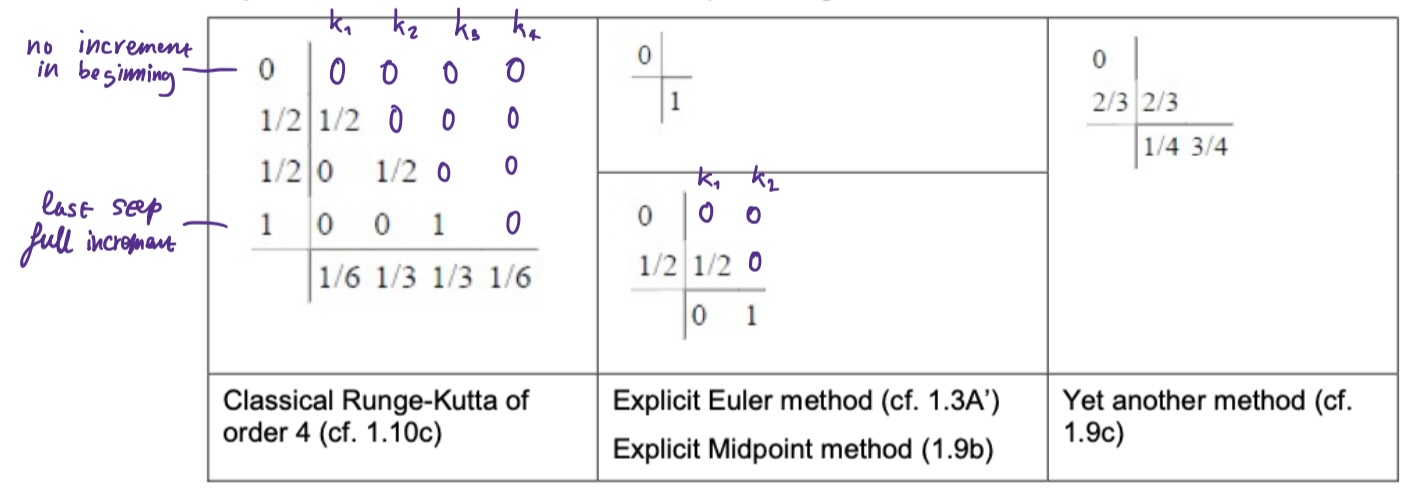
\includegraphics[width=\columnwidth]{images/butcher_tableau}}

\paragraph{FSAL property} (First Same As Last) means that $a_{s,j}=b_j\ (j=1,\ldots,s-1)$
and $b_s = 0$ and $\sum_{j=1}^{s-1}b_j = 1$.
This allows reusing $k_s$ as $k_1$ for the next step.

\subsection{Adaptive Explicit Runge-Kutta Methods}

Use estimates of the local error to adjust the step size $h_i$.
To get an estimate of the local error, we use two different methods of different
\colorbox{shadecolor}{orders $p$ $\hat{p}$},
typically with $\hat{p}=p\mp1$ and noted as $p(\hat{p})$.
They share the \emph{same coefficients matrix} and are called \textbf{embedded methods}.

The combined butcher tableau is:
\begin{align*}
    \begin{array}{c|ccccc}
    {\color{blue}c_1 = 0}
        & {\color{purple}a_{1,1} = 0}
        & {\color{purple}a_{1,2} = 0}
        & {\color{purple}\cdots}
        & {\color{purple}a_{1,{s-1}} = 0}
        & {\color{purple}a_{1,s} = 0}
        \\
        {\color{blue}c_2}
        & {\color{purple}a_{2,1}}
        & {\color{purple}0}
        & {\color{purple}\cdots}
        & {\color{purple}0}
        & {\color{purple}0}
        \\
        {\color{blue}\vdots}
        & {\color{purple}\vdots}
        & {\color{purple}\vdots}
        & {\color{purple}\ddots}
        & {\color{purple}0}
        & {\color{purple}0}
        \\
        {\color{blue}c_{s-1}}
        & {\color{purple}a_{s-1,1}}
        & {\color{purple}a_{s-1,2}}
        & {\color{purple}\cdots}
        & {\color{purple}0}
        & {\color{purple}0}
        \\
        {\color{blue}c_{s}}
        & {\color{purple}a_{s,1}}
        & {\color{purple}a_{s,2}}
        & {\color{purple}\cdots}
        & {\color{purple}a_{s,s-1}}
        & {\color{purple}0}
        \\
        \hline
        & {\color{red}b_1}
        & {\color{red}b_2}
        & {\color{red}\cdots}
        & {\color{red}b_{s-1}}
        & {\color{red}b_s}
        \\
        & {\color{red}\hat{b}_1}
        & {\color{red}\hat{b}_2}
        & {\color{red}\cdots}
        & {\color{red}\hat{b}_{s-1}}
        & {\color{red}\hat{b}_s}
    \end{array}
\end{align*}

and thus receiving two solutions
\begin{align*}
    y_{i+1} & = y_i + h_i\sum_{j=1}^{s}b_jk_j \\
    \hat{y}_{i+1} & = y_i + h_i\sum_{j=1}^{s}\hat{b}_jk_j
\end{align*}

and an estimate for the local error
(double bars indicating norm function when applying to systems of differential equations):
\begin{align*}
    ||e_i||
    = \left|\left|h_i\sum_{j=1}^{s}(b_j-\hat{b}_j)k_j\right|\right|
\end{align*}

We can then implement the following algorithm:
\begin{enumerate}
    \item{
        \emph{Choose an appropriate method}
        (e.g.\ the Heun-Euler method with $p=2$ and $\hat{p}=1$, writing HE2(1)
        where Heun is the primary method and Euler is embedded in Heun).
    }
    \item{
        Choose initial step size $h_0$ and an absolute tolerance $\varepsilon_{a}$ (= accuracy) as
        well as a relative tolerance $\varepsilon_{r}$ (= precision).
        Given accuracy goal $ag$ and precision goal $pg$,
        the tolerances can be computed as \smallshade{$\varepsilon_{a} = 10^{-ag}$}
        and \smallshade{$\varepsilon_{r} = 10^{-pg}$}.
        The errors form the tolerance parameter/error norm
        \colorbox{shadecolor}{
            $\displaystyle\varepsilon = \varepsilon_a + \varepsilon_r |y_n|$
        }
    }
    \item Then start repeating with $i=0$:
    \item{
        \begin{enumerate}
            \item{
                Approximate local error $||e_i||$ and compare it to the error norm $\varepsilon$.
            }
            \item{
                If $||e_i||\leq\varepsilon\ \Rightarrow$ error below tolerance,
                the step is \emph{\color{darkgreen}accepted}.
                We therefore calculate $y_{i+1}$ according to the primary method,
                set $x_{i+1} = x_i + h_i$ and increase $i$.
                We also increase the step size:
                \begin{align*}
                    h_\text{next} = h_{i+1} = h_i\left(\frac{||e_i||}{\varepsilon}\right)^{-\frac{1}{\varrho}}
                \end{align*}
                with $\varrho = \min\{p, \hat{p}\} + 1$ (e.g. 2 for HE2(1))
            }
            \item{
                If $||e_i||>\varepsilon$, the step is \emph{\color{red}rejected}.
                We therefore repeat without increasing $i$ and reduce the step size:
                \begin{align*}
                    h_\text{next} = h_i\left(\frac{||e_i||}{\varepsilon}\right)^{-\frac{1}{\varrho}}
                \end{align*}
                with $\varrho = \min\{p, \hat{p}\} + 1$ (e.g. 2 for HE2(1))
                and $h_\text{next}$ being the step size for the next iteration.
            }
            \item Repeat until desired interval is reached.
        \end{enumerate}
    }
\end{enumerate}

\subsection{Stability of Explicit Runge-Kutta Methods}

Stability refers to the evolution of the global error over time when
continuing using the same step size $h$.

We can benchmark the stability of a method by applying it to the Dahlquist test equation:

\colorbox{shadecolor}{$
\displaystyle
y' = Ay\quad y(0) = 1
$}

with $A\in\mathbb{C}$ or $A$ a constant matrix in case that $y$ is a vector.
The exact solution is $y(t) = e^{At}$, or:
\begin{align*}
    y = e^{\Re(A)x}\left(
    \underbrace{\cos(\omega x) + i\sin(\omega x)}_{\text{oscillating } = e^{i\omega x}}
    \right)
    \quad\text{with }\omega = \Im(A)
\end{align*}

\subsubsection{Example: Absolute stability analysis for Heun's method}

The Heun method is a Runge-Kutta method of order 2 with 2 stages:
\begin{align*}
    & y_0 = y(x_0) \\
    & y_{i+1}=y_{i}+{\frac{1}{2}}h\bigl(f(x_{i},y_{i})+f(x_{i}+h,y_{i}+h f(x_{i},y_{i}))\bigr)
\end{align*}

applied to Dahlquist test equation $y' = Ay$ {\color{gray}($f(x,y) = Ay$)}, the scheme becomes:
\begin{align*}
    y_0 & = y(0) = 1 \\
    y_{i+1} & = y_{i}+{\frac{1}{2}}h\bigl(Ay_{i}+A(y_i + hAy_i)\bigr) \\
    & = \underbrace{\left( 1+hA+\frac{1}{2}(hA)^2 \right)}_{\text{Function }F(hA)=F(z)}y_i \\
    & = F(z)y_i \quad\text{with }z:=hA\text{ and }F(z):=1+z+\frac{1}{2}z^2
\end{align*}

The following stability cases can be distinguished:
\begin{enumerate}
    \item{
        \textbf{Stable} if $\Re(A) < 0$ and thus the solution's amplitude is exponentially decreasing.
        This implies that \colorbox{shadecolor}{$|F(z)| < 1$} for all $z=hA$.
    }
    \item{
        \textbf{Unstable} if $\Re(A) > 0$ and thus the solution's amplitude is exponentially increasing.
        This implies that \colorbox{shadecolor}{$|F(z)| > 1$} for all $z=hA$.
    }
    \item{
        \textbf{Neutral} if $\Re(A) = 0$ and thus the solution's amplitude is constant.
        This implies that \colorbox{shadecolor}{$|F(z)| = 1$} for all $z=hA$ but usually is algebraically hard to achieve.
    }
\end{enumerate}

in the case for Heun's method, we have a stability region of
$hA\in(-2,0)$ for $hA\in\mathbb{R}$.

\subsection{Stiffness}

Stiffness has a negative impact on the stability of a numerical scheme and enforces small step-sizes
leading to high computational costs.

To get a stiffness analysis in a simple, one-dimensional, explicit case, we substitute
$A=\frac{\partial f}{\partial y}$ for the Dahlquist test equation $y'=Ay$.
If we have a bad step size $h$ for a stiff problem then the numerical solution will be outside
of the stability region and thus unstable.
\\[1em]
\textbf{Stiffness detection} for explicit Runge-Kutta methods can be done by using the
approximation

\colorbox{shadecolor}{$
    \displaystyle
    \tilde{\lambda} = \frac{||k_s - k_{s-1}||}{||g_s - g_{s-1}||}
$}

as an estimate for the partial derivative $\frac{\partial f}{\partial y}$ at position $x+h$ provided
that $c_{s-1} = c_s = 1$ for an explicit Runge-Kutta method with at least two $k$ values:
\begin{align*}
    k_{s-1}
    & = f(x+c_{s-1}h,\underbrace{y+h\sum_{j=1}^{s}a_{s-1,j}k_{j}}_{g_{s-1}}) \\
    k_{s}
    & =f(x+c_{s}h,\underbrace{y+h\sum_{j=1}^{s}a_{s,j}k_{j}}_{g_{s}})
\end{align*}

The value $\tilde{\lambda}$ takes the role of $|\Re(A)|$ in the stability analysis.
By testing $|h\tilde\lambda|$ agains the absolute boundary values of the stability region,
we can detect stiffness.

\subsection{Systems of ODEs}
\begin{align*}
    {\vec{y'}}(x)={\vec{f}}(x,{\vec{y}}(x))\quad\text{with }{\vec{y}}(x_0)={\vec{y}}_0\text{ and }m\text{ dimensions}
\end{align*}

We can transform a higher-order ODE by substituting $z_1 = z', z_2 = z'', \ldots, z_{n+1} = h^{(n+1)}$
into a system of first-order ODEs: $z' = z_1, z_1^\prime = z_2, \ldots$
